\section{container.cc File Reference}
\label{container_8cc}\index{container.cc@{container.cc}}
{\tt \#include \char`\"{}container.h\char`\"{}}\par
{\tt \#include $<$dirent.h$>$}\par
{\tt \#include $<$cassert$>$}\par
{\tt \#include $<$cmath$>$}\par
{\tt \#include $<$fstream$>$}\par
{\tt \#include $<$iostream$>$}\par
{\tt \#include \char`\"{}log.h\char`\"{}}\par
{\tt \#include \char`\"{}edge.h\char`\"{}}\par
{\tt \#include \char`\"{}nice.h\char`\"{}}\par
{\tt \#include \char`\"{}controls.h\char`\"{}}\par
{\tt \#include \char`\"{}opttritri.h\char`\"{}}\par
{\tt \#include \char`\"{}Wm4Quaternion.h\char`\"{}}\par
{\tt \#include \char`\"{}vertex\_\-schedule.h\char`\"{}}\par
{\tt \#include \char`\"{}octree\_\-visitor\_\-check\_\-face.h\char`\"{}}\par


Include dependency graph for container.cc:\begin{figure}[H]
\begin{center}
\leavevmode
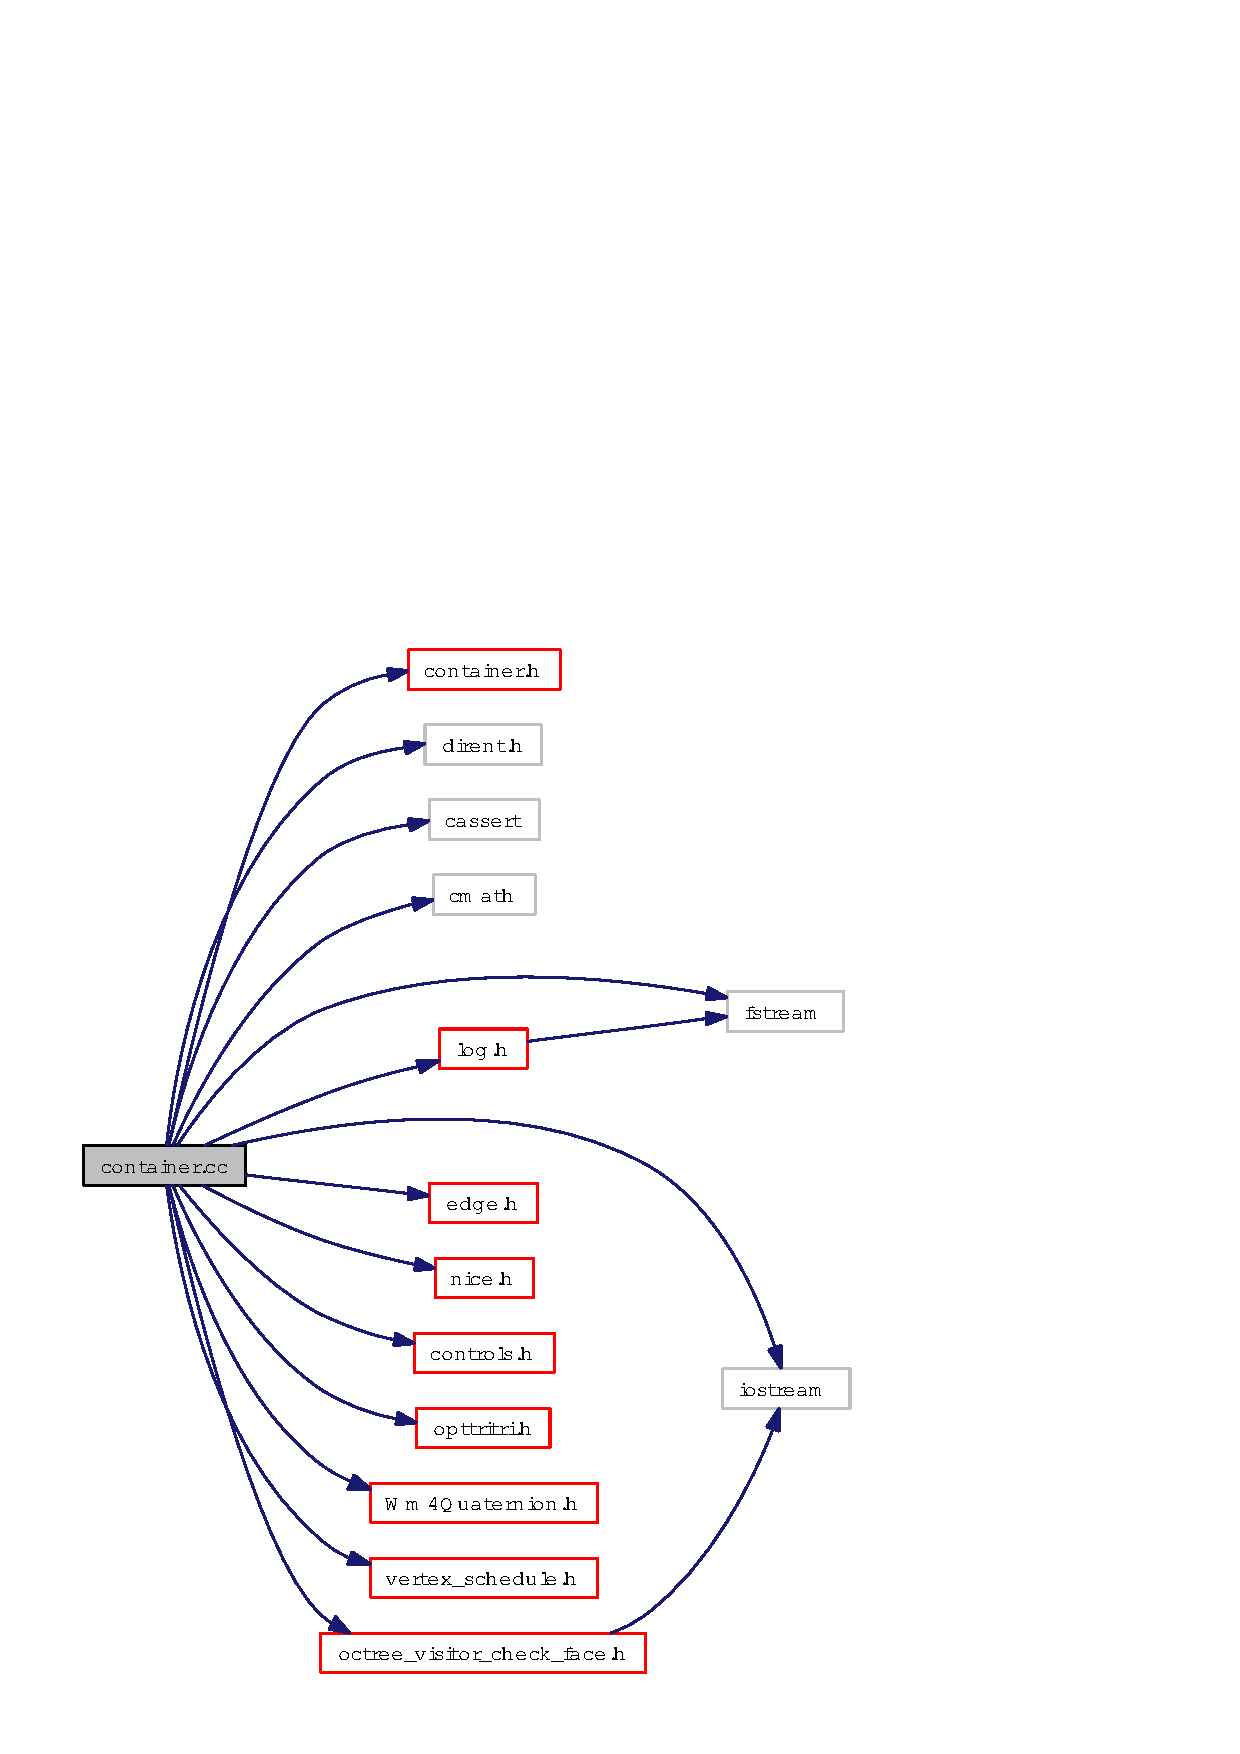
\includegraphics[width=206pt]{container_8cc__incl}
\end{center}
\end{figure}
\subsection*{Functions}
\begin{CompactItemize}
\item 
void {\bf keep\-Min} ({\bf vector3} \&min, {\bf Wm4::Vector3}$<$ double $>$ q)
\item 
void {\bf keep\-Max} ({\bf vector3} \&max, {\bf Wm4::Vector3}$<$ double $>$ q)
\end{CompactItemize}


\subsection{Function Documentation}
\index{container.cc@{container.cc}!keepMax@{keepMax}}
\index{keepMax@{keepMax}!container.cc@{container.cc}}
\subsubsection{\setlength{\rightskip}{0pt plus 5cm}void keep\-Max ({\bf vector3} \& {\em max}, {\bf Wm4::Vector3}$<$ double $>$ {\em q})}\label{container_8cc_751c0c375dacc25e2bab815b767b3fb6}


\index{container.cc@{container.cc}!keepMin@{keepMin}}
\index{keepMin@{keepMin}!container.cc@{container.cc}}
\subsubsection{\setlength{\rightskip}{0pt plus 5cm}void keep\-Min ({\bf vector3} \& {\em min}, {\bf Wm4::Vector3}$<$ double $>$ {\em q})}\label{container_8cc_4ad0271730b851c04d73a2438d7730da}


